% \begin{figure}
%     \centering
%     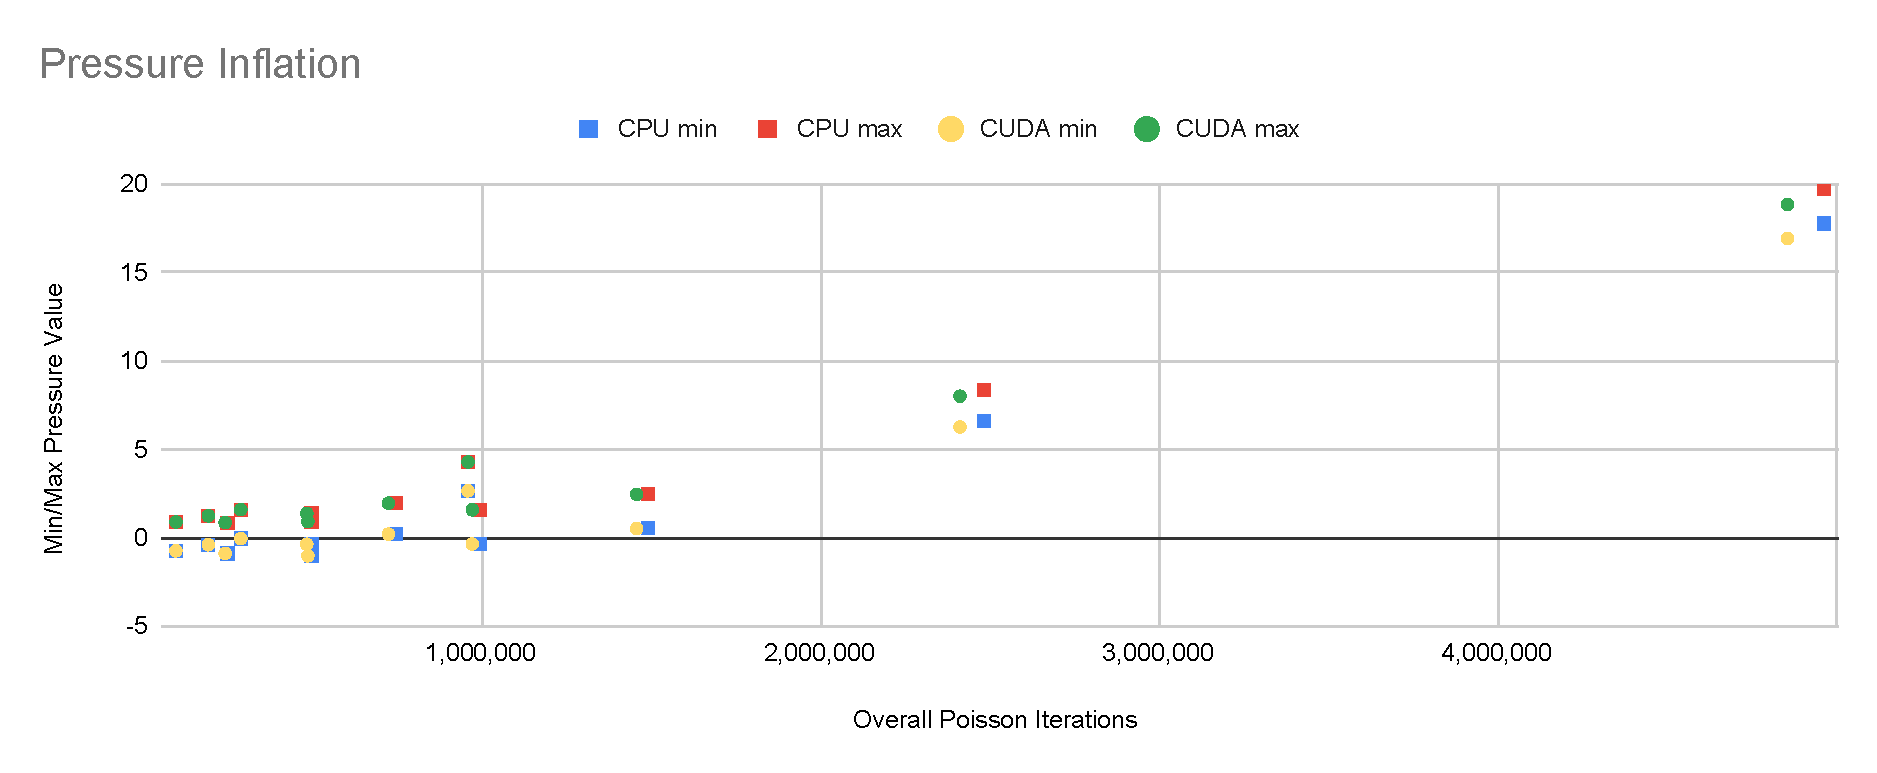
\includegraphics[width=\linewidth]{Ch62Results/figures/temp_pressure_inflation.pdf}
%     \caption{Inflation of pressure values with Poisson iterations}
%     \label{fig:results:pressure_inflation}
% \end{figure}

\begin{figure}
    \centering
    \resizebox{\linewidth}{!}{%
    \begin{tikzpicture}
    \begin{axis}[
        title={Poisson Pressure Inflation},
        ylabel={Pressure Value Range},
        xlabel={Poisson Iterations},
        width=\linewidth,
        height=15em,
        ymin=-5, ymax=25,
        scaled x ticks = false,
        xtick={1000000, 2000000, 3000000, 4000000, 5000000},
        x tick label style={/pgf/number format/fixed},
        xmin=0, xmax=5000000,
        legend pos=north west
    ]
    \addplot+[only marks]%,draw=red] 
        plot [error bars/.cd, y dir=both, y explicit] 
        table [x=iters, y=cpu_mid, y error minus=delta_min_cpu, y error plus=delta_max_cpu, col sep=space, ignore chars={\,}] {Ch62Results/figures/data/pressure_inflation_cpu.csv};
    \addlegendentry{CPU};
    \addplot+[only marks]%,draw=blue] forget plot?
            plot [error bars/.cd, y dir=both, y explicit] 
            table [x=iters, y=cuda_mid, y error plus=delta_max_cuda, y error minus=delta_min_cuda, col sep=space, ignore chars={\,}] {Ch62Results/figures/data/pressure_inflation_cuda.csv};% 
    % \addplot table [x=cache, y=cuda, col sep=space, ignore chars={\,}] {Ch62Results/figures/data/pressure_inflation_cuda.csv};
    \addlegendentry{CUDA};

    \end{axis}
    \end{tikzpicture}
    }
    \caption{Inflation of pressure values with Poisson iterations}
    \label{fig:results:pressure_inflation}
\end{figure}